\documentclass[11pt]{article}
\usepackage[utf8]{inputenc}
\usepackage[a4paper, margin=0.8in]{geometry}
\usepackage{hyperref}
\usepackage{enumitem}
\usepackage{fontawesome5}
\usepackage{xcolor}
\usepackage{titlesec}
\usepackage[skins]{tcolorbox}
\usepackage{fancyhdr}
\usepackage{booktabs}
\usepackage{tikz}
\usepackage{pgfplots}
\pgfplotsset{compat=1.18}

% GitHub colors
\definecolor{githubBlack}{HTML}{24292E}
\definecolor{githubBlue}{HTML}{0366D6}
\definecolor{githubGreen}{HTML}{28A745}
\definecolor{githubPurple}{HTML}{6F42C1}
\definecolor{githubYellow}{HTML}{DBAB09}
\definecolor{githubGray}{HTML}{6A737D}

% Language colors
\definecolor{langC}{HTML}{A8B9CC}
\definecolor{langTypeScript}{HTML}{3178C6}
\definecolor{langCSS}{HTML}{6A737D}
\definecolor{langHTML}{HTML}{6A737D}
\definecolor{langJavaScript}{HTML}{F7DF1E}
\definecolor{langJupyterNotebook}{HTML}{6A737D}

\hypersetup{
  colorlinks=true,
  linkcolor=githubBlue,
  urlcolor=githubBlue,
  pdftitle={GitHub Profile: Lakshya Jain},
  pdfauthor={Lakshya Jain}
}

\titleformat{\section}
  {\normalfont\Large\bfseries\color{githubBlue}}
  {\thesection}
  {1em}
  {}

\pagestyle{fancy}
\fancyhf{}
\renewcommand{\headrulewidth}{0.5pt}
\renewcommand{\footrulewidth}{0.5pt}
\fancyhead[L]{\textcolor{githubBlue}{GitHub Profile: Lakshya Jain}}
\fancyhead[R]{\textcolor{githubGray}{April 14, 2025}}
\fancyfoot[C]{\textcolor{githubGray}{Page \thepage}}

\begin{document}

% Title section
\begin{center}
  \begin{tcolorbox}[
    enhanced,
    colback=githubBlack,
    colframe=githubBlue,
    width=\textwidth,
    arc=4mm,
    boxrule=1.5pt,
    fonttitle=\bfseries
  ]
    {\Huge\textcolor{white}{\faGithub\ Lakshya Jain}}\\[0.3cm]
    {\large\textcolor{githubGray}{GitHub Profile Report \textbullet\ April 14, 2025}}
  \end{tcolorbox}
\end{center}

% Profile Summary
\section*{\faTerminal\ Developer Profile}
\begin{tcolorbox}[
  enhanced,
  colback=black!95,
  colframe=githubGreen!70,
  arc=3mm,
  boxrule=0.5pt,
  fontupper=\ttfamily\color{githubGreen!70}
]
  \begin{itemize}[leftmargin=*, itemsep=0.5em]
    \item \textcolor{githubBlue}{\$} username: \textcolor{white}{lakshya1333}
    \item \textcolor{githubBlue}{\$} name: \textcolor{white}{Lakshya Jain}
    \item \textcolor{githubBlue}{\$} bio: \textcolor{white}{Not provided}
    \item \textcolor{githubBlue}{\$} location: \textcolor{white}{Not provided}
    \item \textcolor{githubBlue}{\$} member since: \textcolor{white}{October 16, 2023}
  \end{itemize}
\end{tcolorbox}

% Coding Languages Radar Chart
\section*{\faCode\ Language Expertise}
\begin{tcolorbox}[
  enhanced,
  colback=githubBlack!10,
  colframe=githubPurple,
  arc=3mm,
  boxrule=0.5pt
]
  \centering
  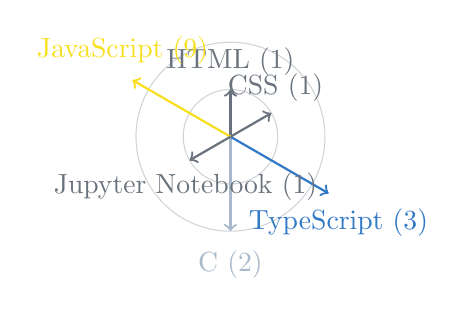
\begin{tikzpicture}[scale=1.2]
    \draw[githubGray!30] (0,0) circle (1);
    \draw[githubGray!30] (0,0) circle (0.5);
    
      \draw[->, thick, langC] (0,0) -- (6.123233995736766e-17,-1);
      \node[anchor=north] at (6.735557395310444e-17,-1.1) {
        \textcolor{langC}{C (2)}
      };
    
      \draw[->, thick, langTypeScript] (0,0) -- (1.0392304845413265,-0.5999999999999999);
      \node[anchor=north] at (1.1431535329954592,-0.6599999999999999) {
        \textcolor{langTypeScript}{TypeScript (3)}
      };
    
      \draw[->, thick, langCSS] (0,0) -- (0.43301270189221935,0.24999999999999997);
      \node[anchor=south] at (0.47631397208144133,0.27499999999999997) {
        \textcolor{langCSS}{CSS (1)}
      };
    
      \draw[->, thick, langHTML] (0,0) -- (3.061616997868383e-17,0.5);
      \node[anchor=south] at (3.367778697655222e-17,0.55) {
        \textcolor{langHTML}{HTML (1)}
      };
    
      \draw[->, thick, langJavaScript] (0,0) -- (-1.0392304845413265,0.5999999999999999);
      \node[anchor=south] at (-1.1431535329954592,0.6599999999999999) {
        \textcolor{langJavaScript}{JavaScript (9)}
      };
    
      \draw[->, thick, langJupyterNotebook] (0,0) -- (-0.4330127018922193,-0.25000000000000006);
      \node[anchor=north] at (-0.4763139720814413,-0.2750000000000001) {
        \textcolor{langJupyterNotebook}{Jupyter Notebook (1)}
      };
    
  \end{tikzpicture}
\end{tcolorbox}

% Contribution Graph
\section*{\faCalendar\ Coding Activity}
\begin{tcolorbox}[
  enhanced,
  colback=white,
  colframe=githubBlack,
  arc=3mm,
  boxrule=0.5pt
]
  \centering
  \begin{tikzpicture}[x=0.15cm, y=0.15cm]
    \fill[RGB,fill={48,161,78}] (0, -0) rectangle +(1,1);
    \fill[RGB,fill={64,196,99}] (0, -1.1) rectangle +(1,1);
    \fill[RGB,fill={33,110,57}] (0, -2.2) rectangle +(1,1);
    \fill[RGB,fill={64,196,99}] (0, -3.3000000000000003) rectangle +(1,1);
    \fill[RGB,fill={48,161,78}] (0, -4.4) rectangle +(1,1);
    \fill[RGB,fill={33,110,57}] (0, -5.5) rectangle +(1,1);
    \fill[RGB,fill={64,196,99}] (0, -6.6000000000000005) rectangle +(1,1);
    \fill[RGB,fill={33,110,57}] (0, -7.700000000000001) rectangle +(1,1);
    \fill[RGB,fill={48,161,78}] (0, -8.8) rectangle +(1,1);
    \fill[RGB,fill={238,238,238}] (0, -9.9) rectangle +(1,1);
    \fill[RGB,fill={155,233,168}] (0, -11) rectangle +(1,1);
    \fill[RGB,fill={48,161,78}] (0, -12.100000000000001) rectangle +(1,1);
    \fill[RGB,fill={155,233,168}] (1.1, -0) rectangle +(1,1);
    \fill[RGB,fill={155,233,168}] (1.1, -1.1) rectangle +(1,1);
    \fill[RGB,fill={48,161,78}] (1.1, -2.2) rectangle +(1,1);
    \fill[RGB,fill={64,196,99}] (1.1, -3.3000000000000003) rectangle +(1,1);
    \fill[RGB,fill={64,196,99}] (1.1, -4.4) rectangle +(1,1);
    \fill[RGB,fill={48,161,78}] (1.1, -5.5) rectangle +(1,1);
    \fill[RGB,fill={33,110,57}] (1.1, -6.6000000000000005) rectangle +(1,1);
    \fill[RGB,fill={238,238,238}] (1.1, -7.700000000000001) rectangle +(1,1);
    \fill[RGB,fill={238,238,238}] (1.1, -8.8) rectangle +(1,1);
    \fill[RGB,fill={33,110,57}] (1.1, -9.9) rectangle +(1,1);
    \fill[RGB,fill={155,233,168}] (1.1, -11) rectangle +(1,1);
    \fill[RGB,fill={155,233,168}] (1.1, -12.100000000000001) rectangle +(1,1);
    \fill[RGB,fill={33,110,57}] (2.2, -0) rectangle +(1,1);
    \fill[RGB,fill={238,238,238}] (2.2, -1.1) rectangle +(1,1);
    \fill[RGB,fill={33,110,57}] (2.2, -2.2) rectangle +(1,1);
    \fill[RGB,fill={238,238,238}] (2.2, -3.3000000000000003) rectangle +(1,1);
    \fill[RGB,fill={64,196,99}] (2.2, -4.4) rectangle +(1,1);
    \fill[RGB,fill={48,161,78}] (2.2, -5.5) rectangle +(1,1);
    \fill[RGB,fill={238,238,238}] (2.2, -6.6000000000000005) rectangle +(1,1);
    \fill[RGB,fill={33,110,57}] (2.2, -7.700000000000001) rectangle +(1,1);
    \fill[RGB,fill={238,238,238}] (2.2, -8.8) rectangle +(1,1);
    \fill[RGB,fill={33,110,57}] (2.2, -9.9) rectangle +(1,1);
    \fill[RGB,fill={48,161,78}] (2.2, -11) rectangle +(1,1);
    \fill[RGB,fill={33,110,57}] (2.2, -12.100000000000001) rectangle +(1,1);
    \fill[RGB,fill={33,110,57}] (3.3000000000000003, -0) rectangle +(1,1);
    \fill[RGB,fill={238,238,238}] (3.3000000000000003, -1.1) rectangle +(1,1);
    \fill[RGB,fill={238,238,238}] (3.3000000000000003, -2.2) rectangle +(1,1);
    \fill[RGB,fill={155,233,168}] (3.3000000000000003, -3.3000000000000003) rectangle +(1,1);
    \fill[RGB,fill={48,161,78}] (3.3000000000000003, -4.4) rectangle +(1,1);
    \fill[RGB,fill={48,161,78}] (3.3000000000000003, -5.5) rectangle +(1,1);
    \fill[RGB,fill={48,161,78}] (3.3000000000000003, -6.6000000000000005) rectangle +(1,1);
    \fill[RGB,fill={33,110,57}] (3.3000000000000003, -7.700000000000001) rectangle +(1,1);
    \fill[RGB,fill={48,161,78}] (3.3000000000000003, -8.8) rectangle +(1,1);
    \fill[RGB,fill={238,238,238}] (3.3000000000000003, -9.9) rectangle +(1,1);
    \fill[RGB,fill={33,110,57}] (3.3000000000000003, -11) rectangle +(1,1);
    \fill[RGB,fill={155,233,168}] (3.3000000000000003, -12.100000000000001) rectangle +(1,1);
    \fill[RGB,fill={33,110,57}] (4.4, -0) rectangle +(1,1);
    \fill[RGB,fill={33,110,57}] (4.4, -1.1) rectangle +(1,1);
    \fill[RGB,fill={64,196,99}] (4.4, -2.2) rectangle +(1,1);
    \fill[RGB,fill={155,233,168}] (4.4, -3.3000000000000003) rectangle +(1,1);
    \fill[RGB,fill={33,110,57}] (4.4, -4.4) rectangle +(1,1);
    \fill[RGB,fill={155,233,168}] (4.4, -5.5) rectangle +(1,1);
    \fill[RGB,fill={48,161,78}] (4.4, -6.6000000000000005) rectangle +(1,1);
    \fill[RGB,fill={155,233,168}] (4.4, -7.700000000000001) rectangle +(1,1);
    \fill[RGB,fill={238,238,238}] (4.4, -8.8) rectangle +(1,1);
    \fill[RGB,fill={64,196,99}] (4.4, -9.9) rectangle +(1,1);
    \fill[RGB,fill={155,233,168}] (4.4, -11) rectangle +(1,1);
    \fill[RGB,fill={155,233,168}] (4.4, -12.100000000000001) rectangle +(1,1);
    \fill[RGB,fill={64,196,99}] (5.5, -0) rectangle +(1,1);
    \fill[RGB,fill={155,233,168}] (5.5, -1.1) rectangle +(1,1);
    \fill[RGB,fill={238,238,238}] (5.5, -2.2) rectangle +(1,1);
    \fill[RGB,fill={155,233,168}] (5.5, -3.3000000000000003) rectangle +(1,1);
    \fill[RGB,fill={48,161,78}] (5.5, -4.4) rectangle +(1,1);
    \fill[RGB,fill={238,238,238}] (5.5, -5.5) rectangle +(1,1);
    \fill[RGB,fill={48,161,78}] (5.5, -6.6000000000000005) rectangle +(1,1);
    \fill[RGB,fill={48,161,78}] (5.5, -7.700000000000001) rectangle +(1,1);
    \fill[RGB,fill={64,196,99}] (5.5, -8.8) rectangle +(1,1);
    \fill[RGB,fill={64,196,99}] (5.5, -9.9) rectangle +(1,1);
    \fill[RGB,fill={48,161,78}] (5.5, -11) rectangle +(1,1);
    \fill[RGB,fill={155,233,168}] (5.5, -12.100000000000001) rectangle +(1,1);
    \fill[RGB,fill={48,161,78}] (6.6000000000000005, -0) rectangle +(1,1);
    \fill[RGB,fill={48,161,78}] (6.6000000000000005, -1.1) rectangle +(1,1);
    \fill[RGB,fill={64,196,99}] (6.6000000000000005, -2.2) rectangle +(1,1);
    \fill[RGB,fill={155,233,168}] (6.6000000000000005, -3.3000000000000003) rectangle +(1,1);
    \fill[RGB,fill={238,238,238}] (6.6000000000000005, -4.4) rectangle +(1,1);
    \fill[RGB,fill={64,196,99}] (6.6000000000000005, -5.5) rectangle +(1,1);
    \fill[RGB,fill={33,110,57}] (6.6000000000000005, -6.6000000000000005) rectangle +(1,1);
    \fill[RGB,fill={33,110,57}] (6.6000000000000005, -7.700000000000001) rectangle +(1,1);
    \fill[RGB,fill={33,110,57}] (6.6000000000000005, -8.8) rectangle +(1,1);
    \fill[RGB,fill={155,233,168}] (6.6000000000000005, -9.9) rectangle +(1,1);
    \fill[RGB,fill={64,196,99}] (6.6000000000000005, -11) rectangle +(1,1);
    \fill[RGB,fill={238,238,238}] (6.6000000000000005, -12.100000000000001) rectangle +(1,1);
    \foreach \y [evaluate=\y as \month using int(\y+1)] in {0,...,11} {
      \node[anchor=east] at (-0.5, -\y*1.1+0.5) {\tiny\textcolor{githubGray}{\month}};
    }
    \node[rotate=90, anchor=south] at (-1.5, -5.5) {\small Months};
    \node[anchor=north] at (3.3, 0.5) {\small Days of Week};
  \end{tikzpicture}
\end{tcolorbox}

% Top Repositories
\section*{\faStar\ Featured Projects}
\begin{tcolorbox}[
  enhanced,
  colback=githubPurple!5,
  colframe=githubPurple,
  arc=3mm,
  boxrule=0.5pt
]
  
    \begin{tcolorbox}[
      enhanced,
      colback=white,
      colframe=githubPurple!30,
      boxrule=0.3pt,
      left=2mm,
      right=2mm,
      top=1mm,
      bottom=1mm,
      overlay={
        \node[anchor=north east, inner sep=1mm] at (frame.north east) 
          {\colorbox{langC}{\textcolor{white}{\scriptsize\bfseries C++}}};
      }
    ]
      \textbf{\textcolor{githubPurple}{Banking-System}} \hfill \textcolor{githubYellow}{1 \faStar}\\
      \small Created using C++ and OOPS concept\\
      \vspace{2mm}
      \begin{flushright}
        \textcolor{githubGray}{\scriptsize\faCodeFork\ 1 \hspace{2mm}\faEye\ 99}
      \end{flushright}
    \end{tcolorbox}
  
\vspace{2mm}

    \begin{tcolorbox}[
      enhanced,
      colback=white,
      colframe=githubPurple!30,
      boxrule=0.3pt,
      left=2mm,
      right=2mm,
      top=1mm,
      bottom=1mm,
      overlay={
        \node[anchor=north east, inner sep=1mm] at (frame.north east) 
          {\colorbox{langC}{\textcolor{white}{\scriptsize\bfseries C}}};
      }
    ]
      \textbf{\textcolor{githubPurple}{OS-Lab}} \hfill \textcolor{githubYellow}{0 \faStar}\\
      \small No description available\\
      \vspace{2mm}
      \begin{flushright}
        \textcolor{githubGray}{\scriptsize\faCodeFork\ 1 \hspace{2mm}\faEye\ 98}
      \end{flushright}
    \end{tcolorbox}
  
\vspace{2mm}

    \begin{tcolorbox}[
      enhanced,
      colback=white,
      colframe=githubPurple!30,
      boxrule=0.3pt,
      left=2mm,
      right=2mm,
      top=1mm,
      bottom=1mm,
      overlay={
        \node[anchor=north east, inner sep=1mm] at (frame.north east) 
          {\colorbox{langUnknown}{\textcolor{white}{\scriptsize\bfseries Unknown}}};
      }
    ]
      \textbf{\textcolor{githubPurple}{Progress-tracker}} \hfill \textcolor{githubYellow}{0 \faStar}\\
      \small tracks progress\\
      \vspace{2mm}
      \begin{flushright}
        \textcolor{githubGray}{\scriptsize\faCodeFork\ 1 \hspace{2mm}\faEye\ 32}
      \end{flushright}
    \end{tcolorbox}
  
\vspace{2mm}

    \begin{tcolorbox}[
      enhanced,
      colback=white,
      colframe=githubPurple!30,
      boxrule=0.3pt,
      left=2mm,
      right=2mm,
      top=1mm,
      bottom=1mm,
      overlay={
        \node[anchor=north east, inner sep=1mm] at (frame.north east) 
          {\colorbox{langTypeScript}{\textcolor{white}{\scriptsize\bfseries TypeScript}}};
      }
    ]
      \textbf{\textcolor{githubPurple}{Mental-Health-SDT-project}} \hfill \textcolor{githubYellow}{0 \faStar}\\
      \small No description available\\
      \vspace{2mm}
      \begin{flushright}
        \textcolor{githubGray}{\scriptsize\faCodeFork\ 1 \hspace{2mm}\faEye\ 54}
      \end{flushright}
    \end{tcolorbox}
  
\vspace{2mm}

    \begin{tcolorbox}[
      enhanced,
      colback=white,
      colframe=githubPurple!30,
      boxrule=0.3pt,
      left=2mm,
      right=2mm,
      top=1mm,
      bottom=1mm,
      overlay={
        \node[anchor=north east, inner sep=1mm] at (frame.north east) 
          {\colorbox{langCSS}{\textcolor{white}{\scriptsize\bfseries CSS}}};
      }
    ]
      \textbf{\textcolor{githubPurple}{My-Portfolio}} \hfill \textcolor{githubYellow}{0 \faStar}\\
      \small No description available\\
      \vspace{2mm}
      \begin{flushright}
        \textcolor{githubGray}{\scriptsize\faCodeFork\ 1 \hspace{2mm}\faEye\ 71}
      \end{flushright}
    \end{tcolorbox}
  
\end{tcolorbox}

% Stats
\section*{\faChartLine\ Development Stats}
\begin{tcolorbox}[
  enhanced,
  colback=githubBlack!5,
  colframe=githubBlue,
  arc=3mm,
  boxrule=0.5pt
]
  \begin{itemize}[leftmargin=*, itemsep=1em]
    \item \textbf{\textcolor{githubBlue}{Total Contributions}} 
      
\begin{tikzpicture}[baseline=-0.5ex]
        \draw[githubBlue!30, very thick] (0,0) -- (5,0);
        \draw[githubBlue, very thick] (0,0) -- (0.05,0);
        \node[anchor=west] at (5.2,0) {\small 2+};
      \end{tikzpicture}
    
    \item \textbf{\textcolor{githubGreen}{Code Output}} 
      
\begin{tikzpicture}[baseline=-0.5ex]
        \draw[githubGreen!30, very thick] (0,0) -- (5,0);
        \draw[githubGreen, very thick] (0,0) -- (2.7,0);
        \node[anchor=west] at (5.2,0) {\small 27 repos};
      \end{tikzpicture}
    
    \item \textbf{\textcolor{githubPurple}{Community Impact}} 
      
\begin{tikzpicture}[baseline=-0.5ex]
        \draw[githubPurple!30, very thick] (0,0) -- (5,0);
        \draw[githubPurple, very thick] (0,0) -- (0.4,0);
        \node[anchor=west] at (5.2,0) {\small 5 followers, 1 forks};
      \end{tikzpicture}
  \end{itemize}
\end{tcolorbox}

% Footer
\vspace{1cm}
\begin{center}
  \begin{tcolorbox}[
    enhanced,
    colback=githubBlack,
    colframe=githubBlue,
    width=0.8\textwidth,
    arc=3mm,
    boxrule=0.5pt
  ]
    \centering
    \small\textcolor{white}{This profile was automatically generated from GitHub data}\\
    \href{https://github.com/lakshya1333}{\textcolor{githubBlue}{\faGithub\ github.com/lakshya1333}}\\
    \textcolor{githubGray}{\scriptsize Generated on April 14, 2025}
  \end{tcolorbox}
\end{center}

\end{document}